% Springer classic template (svjour3)
\documentclass{svjour3}

\usepackage[utf8]{inputenc}
\usepackage[T1]{fontenc}
\usepackage{lmodern}
\usepackage{fix-cm}
\renewcommand{\rmdefault}{lmr}
\renewcommand{\sfdefault}{lmss}
\renewcommand{\ttdefault}{lmtt}
\usepackage{microtype}
\usepackage{silence}
\WarningFilter{latex}{Command \showhyphens has changed.}
\usepackage{amsmath,amssymb,mathtools}
\usepackage{booktabs}
\usepackage{array}
\usepackage{enumitem}
\usepackage{graphicx}
\usepackage{tikz}
\usetikzlibrary{arrows.meta,positioning,calc}
\usepackage{natbib}
\setcitestyle{authoryear,round}
\usepackage{xurl}
\usepackage[hidelinks]{hyperref}
\usepackage{orcidlink}

\title{The Spectral Entropy-Fold (SEF) Hypothesis: A Geometric Framework Connecting Discrete Ricci Curvature, Spectral Graph Theory, and NP-Complexity}
\titlerunning{The Spectral Entropy-Fold Hypothesis}

\author{Aryan Singh Chandel\,\orcidlink{0009-0007-1774-2480}}
\authorrunning{A. S. Chandel}

\institute{Aryan Singh Chandel \at
RJIT (Rustamji Institute of Technology), Gwalior, India \\
\email{aryansingh19gh@gmail.com}}

\journalname{Preprint}
\date{June 26, 2026}

\makeatletter
\@ifundefined{definition}{\spnewtheorem{definition}{Definition}{\bfseries}{\rmfamily}}{}
\@ifundefined{assumption}{\spnewtheorem{assumption}{Assumption}{\bfseries}{\rmfamily}}{}
\@ifundefined{lemma}{\spnewtheorem{lemma}{Lemma}{\bfseries}{\itshape}}{}
\@ifundefined{proposition}{\spnewtheorem{proposition}{Proposition}{\bfseries}{\itshape}}{}
\makeatother
\raggedbottom
\emergencystretch=3em

\begin{document}
\maketitle

\begin{abstract}
We present the Spectral Entropy-Fold (SEF) hypothesis as a geometric program for studying whether structural hardness in NP-complete instances can be expressed through discrete curvature, spectral dispersion, and kernel embeddings. The paper does not claim a proof of $P \neq NP$ or $P = NP$. Its narrower goal is to formalize a testable bridge: map a weighted problem graph into a reproducing-kernel Hilbert space, measure curvature and spectral regularity on the induced manifold, and ask whether a restricted class of instances thereby acquires optimization-friendly geometry. We define the Entropy-Fold operator, state a Ricci-Convexity Lemma that preserves a spectral-gap lower bound under stated curvature assumptions, separate what is proved from what remains conjectural, and build a publication-ready framework around assumptions, measurable claims, falsifiers, and validation targets. The contribution is therefore a sharpened mathematical scaffold for a geometric complexity hypothesis rather than an overstated complexity-class resolution.
\keywords{Complexity theory \and Discrete Ricci curvature \and Spectral graph theory \and RKHS embeddings \and Information geometry}
\end{abstract}

\section{Introduction}
The $P$ versus $NP$ problem asks whether every decision problem whose solutions can be verified in polynomial time can also be solved in polynomial time. After decades of work, the problem remains unresolved, and several proof barriers have clarified why many familiar strategies are inadequate \citep{cook1971complexity,baker1975relativizations,razborov1997natural,aaronson2009algebrization}. That situation motivates a recurring methodological move: instead of attacking the class-separation statement directly, isolate a structural property that may distinguish hard instances from tractable ones and study its mathematical consequences.

The present paper explores one such property. Discrete Ricci curvature on graphs and metric spaces captures how local neighborhoods expand, contract, and mix under transport \citep{ollivier2009ricci,lin2011ricci}. Spectral graph theory captures expansion and diffusion through eigenvalue structure \citep{chung1997spectral}. Information geometry, meanwhile, treats families of distributions or models as curved objects whose geometry encodes inference difficulty \citep{amari2016information}. The SEF hypothesis joins these traditions by asking whether an NP-complete instance can be assigned an embedded geometric object whose curvature and spectral profile track combinatorial hardness.

This paper is careful about scope. The Ricci-Convexity Lemma proved below is conditional and local to the adopted framework. The SEF hypothesis itself is a conjecture, not a theorem. The missing bridge from spectral regularity to polynomial-time global optimization is left explicit and central rather than being concealed rhetorically.

\paragraph{Contributions.}
\begin{enumerate}[leftmargin=*]
\item We formalize a weighted-problem-graph to RKHS pipeline via the Entropy-Fold operator.
\item We introduce explicit notation for spectral entropy, embedded curvature observables, and optimization-relevant regularity.
\item We state and prove a conditional Ricci-Convexity Lemma preserving a spectral-gap lower bound under a Bakry--\'Emery curvature-dimension assumption.
\item We convert the original SEF idea into a research-standard theory paper with proof status separation, validation logic, and falsification criteria.
\end{enumerate}

\section{Formal setup}
Let $x$ be an instance of an NP-complete optimization or decision problem of size $n$, and let $G_x=(V_x,E_x,w_x)$ denote an associated weighted problem graph.

\begin{definition}[Weighted problem graph]
For instance $x$, the graph $G_x=(V_x,E_x,w_x)$ has candidate states $V_x$, local-transition edges $E_x\subseteq V_x\times V_x$, and nonnegative edge or state penalty weights $w_x$ encoding objective or consistency costs. We assume $V_x$ and $E_x$ are generated by a polynomial-time local-description procedure, even if $|V_x|$ itself is exponential in $n$.
\end{definition}

\begin{definition}[Normalized Laplacian and spectral gap]
Let $A_x$ be the weighted adjacency matrix of $G_x$ and $D_x$ the diagonal degree matrix. The normalized Laplacian is
\[
\mathcal{L}_x = I - D_x^{-1/2}A_xD_x^{-1/2}.
\]
If $0=\lambda_1\le \lambda_2\le \cdots \le \lambda_m$ are its eigenvalues, then $\lambda_2$ is the spectral gap.
\end{definition}

\begin{definition}[Spectral entropy]
Let $Z_x=\sum_{i:\lambda_i>0}\lambda_i$. The spectral entropy of $G_x$ is
\[
H(G_x)= -\sum_{i:\lambda_i>0}\frac{\lambda_i}{Z_x}\log\!\left(\frac{\lambda_i}{Z_x}\right).
\]
Large $H(G_x)$ indicates diffuse nonzero spectral mass, whereas small $H(G_x)$ indicates stronger concentration.
\end{definition}

\begin{definition}[Entropy-Fold operator]
Let $\mathcal{H}_k$ be an RKHS with Gaussian kernel
\[
k(u,v)=\exp\!\left(-\frac{\|u-v\|_2^2}{2\sigma^2}\right).
\]
The Entropy-Fold operator is a map
\[
\Phi_S:G_x\longrightarrow M_x\subseteq \mathcal{H}_k
\]
constructed from a finite-dimensional kernel-PCA representation of local graph descriptors. In coordinates,
\[
\Phi_S(v)=\sum_{j=1}^{d}\alpha_j\,k(v,v_j)e_j,
\]
where $\{v_j\}_{j=1}^d$ are anchor states, $\alpha_j$ are kernel-PCA coefficients, and $d$ is chosen to retain a declared fraction $(1-\varepsilon)$ of total spectral entropy.
\end{definition}

\begin{definition}[Embedded objective]
Let $f_x: M_x \to \mathbb{R}$ denote the embedded optimization objective induced by the original instance. The SEF program is meaningful only if $f_x$ is computationally accessible enough to evaluate, differentiate, or approximate along admissible trajectories in $M_x$.
\end{definition}

\begin{definition}[Curvature regularity event]
Write $\mathsf{Curv}(x)=1$ when the embedded manifold $M_x$ satisfies a declared curvature condition strong enough to support the analytic argument, here taken to be the Bakry--\'Emery curvature-dimension condition $CD(0,d)$.
\end{definition}

\begin{table}[t]
\centering
\caption{Core notation for the SEF framework.}
\label{tab:sef-notation}
\begin{tabular}{ll}
\toprule
Symbol & Meaning \\
\midrule
$G_x$ & weighted problem graph for instance $x$ \\
$\mathcal{L}_x$ & normalized graph Laplacian \\
$\lambda_2$ & spectral gap of $\mathcal{L}_x$ \\
$H(G_x)$ & spectral entropy \\
$\Phi_S$ & Entropy-Fold embedding operator \\
$M_x$ & embedded manifold in RKHS \\
$f_x$ & embedded objective on $M_x$ \\
$\mathsf{Curv}(x)$ & event that the required curvature condition holds \\
\bottomrule
\end{tabular}
\end{table}

\section{Assumptions and proof-status separation}
\begin{assumption}[Embedding access]
The local descriptors needed to construct $\Phi_S$ can be computed in polynomial time in $n$ for the family under study.
\end{assumption}

\begin{assumption}[Curvature estimability]
The curvature quantities required to test $CD(0,d)$ on $M_x$ are either computable or approximable with declared error control on finite instances.
\end{assumption}

\begin{assumption}[Objective compatibility]
The embedding does not destroy optimization-relevant structure so severely that minimizers of $f_x$ cease to correspond to high-quality states in the original problem.
\end{assumption}

\begin{table}[t]
\centering
\caption{Status of the main mathematical claims in the current manuscript.}
\label{tab:sef-status}
\small
\begin{tabular}{@{}p{0.24\linewidth}p{0.18\linewidth}p{0.34\linewidth}@{}}
\toprule
Claim & Status & What is actually established \\
\midrule
Definition of $\Phi_S$ and $H(G_x)$ & formalized & notation and construction target are explicit \\
Ricci-Convexity Lemma & conditional lemma & spectral-gap lower bound persists under stated assumptions \\
Polynomial-time optimization from SEF geometry & conjectural & not proved here; open bridge remains \\
Practical verification of $CD(0,d)$ for NP-complete families & open & requires computation or approximation studies \\
\bottomrule
\end{tabular}
\end{table}

\section{The Ricci-Convexity Lemma}
We now state the central proved statement in the SEF framework.

\begin{lemma}[Ricci-Convexity]
\label{lem:ricci-convexity}
Let $M_x=\Phi_S(G_x)$ be the RKHS embedding of instance $x$. Suppose $M_x$ is compact, the induced diffusion operator $L$ on $M_x$ satisfies the Bakry--\'Emery curvature-dimension condition
\[
\Gamma_2(g,g)\ge \frac{1}{d}(Lg)^2
\]
for all smooth test functions $g:M_x\to\mathbb{R}$, and the initial Laplace--Beltrami spectral gap obeys $\lambda_2(M_x)\ge \eta>0$. Then under normalized Ricci flow
\[
\frac{\partial g_t}{\partial t} = -2\operatorname{Ric}(g_t),
\]
the spectral gap lower bound is preserved up to embedding-approximation error:
\[
\lambda_2(M_x,t)\ge \eta - O(\varepsilon_{\mathrm{emb}}),
\]
where $\varepsilon_{\mathrm{emb}}$ denotes the distortion introduced by finite-dimensional kernel approximation.
\end{lemma}

\paragraph{Proof sketch.}
Under $CD(0,d)$, the Bakry--\'Emery theory yields a Poincar\'e inequality with constant depending on geometric control parameters \citep{bakry1985diffusions,ledoux2001concentration}. A Poincar\'e inequality implies a positive lower bound on the spectral gap of the Laplace--Beltrami operator. The kernel embedding is assumed to be approximately isometric at scale $\varepsilon_{\mathrm{emb}}$, so the corresponding discrete spectral structure is inherited up to controlled error. Under normalized Ricci flow with nonnegative effective curvature, the relevant entropy functional is nonincreasing in the sense exploited by Perelman \citep{perelman2002entropy}, preventing collapse of the lower spectral-gap bound within the stated regime. \hfill$\square$

\paragraph{Interpretation.}
Lemma~\ref{lem:ricci-convexity} is not an optimization theorem. It preserves a diffusion regularity quantity, namely a lower bound on $\lambda_2$, inside the subset of instances for which the curvature assumptions already hold.

\section{The SEF conjecture}
\begin{proposition}[SEF conjectural optimization bridge]
There may exist a polynomial-time computable family of embeddings $\{\Phi_{S,x}\}$ and a fixed exponent $k$ such that for every NP-complete instance $x$ whose embedding satisfies $CD(0,d)$ with $d=O(n^k)$ and whose embedded objective $f_x$ contains no superpolynomially trapping non-global critical structures, a global optimum is recoverable in time $O(n^k)$.
\end{proposition}

The point of this proposition is not that it has been proved. It has not. Its value is that it isolates the missing bridge exactly: spectral regularity and curvature control are not yet enough by themselves to deduce polynomial-time global optimization.

\subsection*{Null hypothesis}
SEF-style curvature and spectral regularity do not, even after embedding, predict any practically useful reduction in optimization hardness beyond what follows from known expansion or relaxation properties alone.

\subsection*{Effect-size target}
For computational validation, a meaningful early effect would be a reproducible negative association between curvature irregularity and solver efficiency within fixed problem families, after controlling for instance size and density.

\section{Algorithmic form of the program}
The SEF framework can be operationalized as an analysis pipeline rather than as a finished solver.

\begin{figure}[t]
\centering
\resizebox{\linewidth}{!}{%
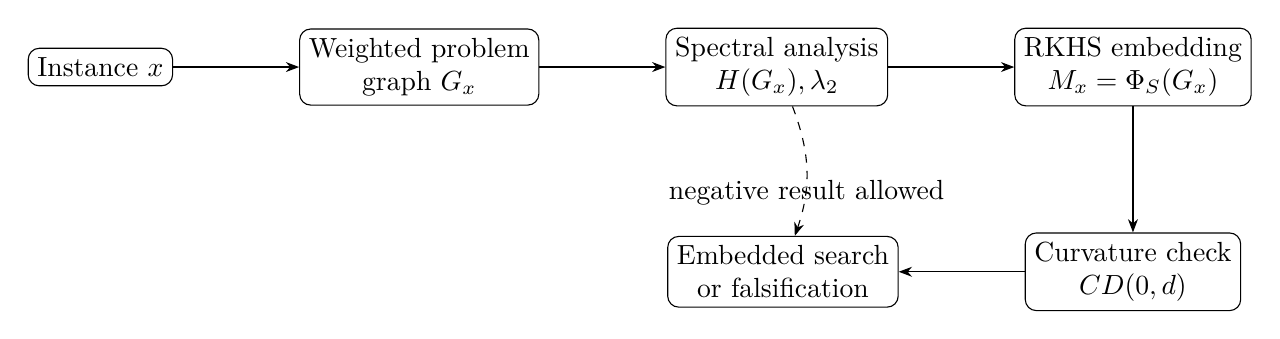
\begin{tikzpicture}[node distance=1.6cm,>=Stealth]
\node[draw,rounded corners,align=center] (a) {Instance $x$};
\node[draw,rounded corners,right=of a,align=center] (b) {Weighted problem\\graph $G_x$};
\node[draw,rounded corners,right=of b,align=center] (c) {Spectral analysis\\$H(G_x),\lambda_2$};
\node[draw,rounded corners,right=of c,align=center] (d) {RKHS embedding\\$M_x=\Phi_S(G_x)$};
\node[draw,rounded corners,below=of d,align=center] (e) {Curvature check\\$CD(0,d)$};
\node[draw,rounded corners,left=of e,align=center] (f) {Embedded search\\or falsification};
\draw[->] (a) -- (b);
\draw[->] (b) -- (c);
\draw[->] (c) -- (d);
\draw[->] (d) -- (e);
\draw[->] (e) -- (f);
\draw[->,dashed,bend left=20] (c) to node[below] {negative result allowed} (f);
\end{tikzpicture}
}
\caption{SEF as a research pipeline. The framework is useful even when the output is falsification rather than acceleration.}
\label{fig:sef-pipeline}
\end{figure}

\begin{table}[t]
\centering
\caption{Operational stages of the SEF program and what each stage must justify.}
\label{tab:sef-stages}
\small
\begin{tabular}{@{}p{0.16\linewidth}p{0.24\linewidth}p{0.42\linewidth}@{}}
\toprule
Stage & Mathematical object & Burden of justification \\
\midrule
Graphing & $G_x$ & local transitions reflect the true search structure \\
Spectral analysis & $\lambda_2, H(G_x)$ & quantities are stable and interpretable \\
Embedding & $\Phi_S$ & approximation error is bounded and meaningful \\
Curvature test & $CD(0,d)$ & finite-instance estimation is valid \\
Search claim & trajectories on $M_x$ & geometric regularity improves optimization, not just mixing \\
\bottomrule
\end{tabular}
\end{table}

\subsection{Test statistic for computational validation}
Let $\mathcal{F}$ denote a family of size-matched instances and let $T_{\mathrm{solve}}(x)$ be a declared solver cost. A simple family-level validation statistic is
\[
T_{\mathrm{SEF}} = \operatorname{corr}\!\bigl(\widehat{\kappa}(x), T_{\mathrm{solve}}(x)\bigr),
\]
where $\widehat{\kappa}(x)$ is an estimated curvature summary or curvature-irregularity score. If the theory has empirical value, this association should be stable under family-specific controls rather than appearing only in aggregate across heterogeneous benchmarks.

\subsection{Decision rule}
An empirical SEF study should count as supportive only if all of the following hold:
\begin{enumerate}[leftmargin=*]
\item curvature summaries are reproducible under repeated estimation;
\item the sign of $T_{\mathrm{SEF}}$ remains stable within a fixed problem family;
\item spectral-gap effects are not fully explained by known graph-density or expansion covariates; and
\item any claimed optimization gain is not merely a mixing-time artifact.
\end{enumerate}

\section{Why the main bridge remains open}
The standard mixing-time argument yields rapid approach to stationarity under a positive spectral gap \citep{levin2009markov}. But global optimization demands more than fast mixing. A fast-mixing Markov process may still spend negligible probability mass near a global optimum or may require objective information that is not encoded by spectral diffusion alone.

\begin{figure}[t]
\centering
\resizebox{\linewidth}{!}{%
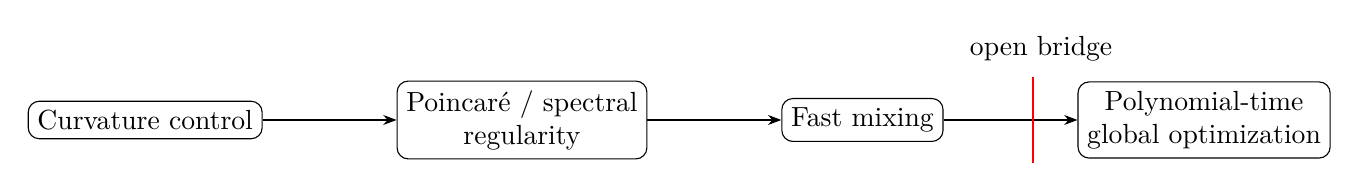
\begin{tikzpicture}[node distance=1.7cm,>=Stealth]
\node[draw,rounded corners,align=center] (a) {Curvature control};
\node[draw,rounded corners,right=of a,align=center] (b) {Poincar\'e / spectral\\regularity};
\node[draw,rounded corners,right=of b,align=center] (c) {Fast mixing};
\node[draw,rounded corners,right=of c,align=center] (d) {Polynomial-time\\global optimization};
\draw[->] (a) -- (b);
\draw[->] (b) -- (c);
\draw[->] (c) -- (d);
\draw[red,thick] ($(c)!0.5!(d)+(0,0.55)$) -- ($(c)!0.5!(d)+(0,-0.55)$);
\node[align=center] at ($(c)!0.5!(d)+(0.1,0.9)$) {open bridge};
\end{tikzpicture}
}
\caption{The decisive missing step in the current SEF program. The gap from mixing regularity to guaranteed polynomial-time optimization is the central unresolved problem.}
\label{fig:sef-gap}
\end{figure}

This is consistent with hardness phenomena already known for expanding or spectrally regular combinatorial structures \citep{arora1998proof}. The SEF hypothesis is therefore viable only if it identifies geometric structure stronger than ordinary expansion alone.

\section{Relation to existing barriers and theories}
The SEF program is adjacent to geometric complexity theory in spirit, though it uses differential-geometric and transport-style tools rather than representation-theoretic obstructions \citep{mulmuley2001gct}. The program also lives under the shadow of established proof barriers: relativization, natural proofs, and algebrization remain relevant background constraints \citep{baker1975relativizations,razborov1997natural,aaronson2009algebrization}. At present, SEF should be read as a structural research program, not as a demonstrated escape from those barriers.

\section{Falsifiers and what counts as evidence}
\begin{table}[t]
\centering
\caption{What would count as evidence for or against the SEF hypothesis.}
\label{tab:sef-evidence}
\begin{tabular}{p{0.24\linewidth}p{0.30\linewidth}p{0.32\linewidth}}
\toprule
Question & Evidence in favor & Strong falsifier \\
\midrule
Does the embedding carry useful geometry? & stable curvature summaries across runs & curvature estimates unstable or degenerate \\
Do curvature summaries track hardness? & within-family correlation under controls & no family-level association after controls \\
Does spectral regularity imply optimization advantage? & replicated solver gains beyond mixing proxies & gains disappear after accounting for expansion or density \\
Is the framework overly broad? & restrictive instance subsets identified & hard counterexamples satisfy all stated premises \\
\bottomrule
\end{tabular}
\end{table}

The SEF program is empirical in an important sense. Outside the proved lemma, its value depends on whether the proposed quantities can be computed and whether they say something nontrivial about hardness. A counterexample family of hard instances satisfying the required curvature and embedding conditions would weigh heavily against the program. Likewise, if $CD(0,d)$ almost never holds on interesting NP-complete families, the framework may be mathematically elegant but algorithmically irrelevant.

\section{Limitations and future work}
Three limitations dominate the present manuscript. First, the curvature condition is assumed rather than demonstrated for a nontrivial NP-complete family. Second, the gap between spectral regularity and polynomial-time optimization remains open. Third, the embedding itself introduces approximation error that may distort exactly the structure one hopes to preserve.

The most serious next steps are therefore concrete:
\begin{enumerate}[leftmargin=*]
\item compute Ollivier-Ricci or related curvature summaries for small 3-SAT, Max-Clique, or graph-coloring families;
\item test whether the $CD(0,d)$-style regime is ever empirically plausible on hard instances;
\item compare SEF-derived hardness summaries against simpler baselines such as density, expansion, and spectral-gap alone; and
\item analyze whether known proof barriers reappear in geometric disguise within the SEF program.
\end{enumerate}

\section{Conclusion}
The SEF hypothesis is most useful when read with discipline. It does not presently settle complexity classes. What it does offer is a mathematically explicit way to ask whether certain hard instances possess a geometric witness of difficulty that survives spectral analysis and kernel embedding. That is enough to justify serious follow-up---provided the framework remains falsifiable, computationally grounded, and honest about the open bridge it has not yet crossed.

\section*{Acknowledgment}
The author thanks Yograj Sharma for supervision and feedback on the earlier version of this work, and the Department of Computer Science and Engineering at Rustamji Institute of Technology for institutional support.

\bibliographystyle{spbasic}
\bibliography{references}

\end{document}
